\def\year{2020}\relax
\documentclass[letterpaper]{article} % DO NOT CHANGE THIS
\usepackage{aaai20}  % DO NOT CHANGE THIS
\usepackage{times}  % DO NOT CHANGE THIS
\usepackage{helvet} % DO NOT CHANGE THIS
\usepackage{courier}  % DO NOT CHANGE THIS
\usepackage[hyphens]{url}  % DO NOT CHANGE THIS
\usepackage{graphicx} % DO NOT CHANGE THIS
\urlstyle{rm} % DO NOT CHANGE THIS
\def\UrlFont{\rm}  % DO NOT CHANGE THIS
\usepackage{graphicx}  % DO NOT CHANGE THIS
\frenchspacing  % DO NOT CHANGE THIS
\setlength{\pdfpagewidth}{8.5in}  % DO NOT CHANGE THIS
\setlength{\pdfpageheight}{11in}  % DO NOT CHANGE THIS
\usepackage{times}
\usepackage{soul}
\usepackage{url}
\usepackage[hidelinks]{hyperref}
\usepackage[utf8]{inputenc}
\usepackage[small]{caption}
\usepackage{graphicx}
\usepackage{amsmath}
\usepackage{booktabs}
\usepackage{amsmath}
\usepackage{amssymb}
\usepackage{mathrsfs}
\usepackage{xcolor}
\usepackage{soul}
\usepackage{amsfonts}
\usepackage{graphicx}
\usepackage{framed}
\usepackage{tikz}
\usetikzlibrary{arrows,shapes.geometric,shapes.arrows}
\usepackage{pgfplots}
\usepackage{amsthm}
\usepackage[ruled,vlined,linesnumbered]{algorithm2e}
\usepackage{makecell}
\usepackage{tikz}
\usepackage{comment}
\urlstyle{same}
\usepackage{multirow}

\usepackage{times}
\usepackage{helvet}
\usepackage{courier}
\usepackage{amsthm}

\usepackage{amssymb,amsthm, amsfonts}

\newtheorem{theorem}{Theorem}
\newtheorem{definition}{Definition}
\newtheorem{observation}{Observation}
\newtheorem{corollary}{Corollary}
\newtheorem{lemma}{Lemma}
\newtheorem{example}{Example}
\newtheorem{conjecture}{Conjecture}
\usepackage[ruled,linesnumbered]{algorithm2e}
\newcommand{\var}{\texttt}



\usepackage{mathtools} % Bonus

\usepackage{lipsum}
\usepackage{csquotes}
\usepackage{verbatim}
\usepackage{tikz}

\usepackage{array,multirow,graphicx}

\usepackage{url}
\newcommand{\commentout}[1]{}

\definecolor{Blue}{rgb}{0,0.16,0.90}
\definecolor{Red}{rgb}{0.90,0.16,0}
\definecolor{DarkBlue}{rgb}{0,0.08,0.45}
\definecolor{ChangedColor}{rgb}{0.9,0.08,0}
\definecolor{CommentColor}{rgb}{0.2,0.8,0.2}
\definecolor{ToDoColor}{rgb}{0.1,0.2,1}

\definecolor{verylightgray}{rgb}{0.91,0.91,0.91}

\newcommand{\todo}[1]{\textbf{\color{ToDoColor} TODO: #1}}
\newcommand{\tal}[1]{\footnote{\textbf{\color{CommentColor} /* #1   (tal)*/}}}
\newcommand{\liat}[1]{\footnote{\textbf{\color{CommentColor} /* #1   (liat)*/}}}
\newcommand{\roni}[1]{\footnote{\textbf{\color{CommentColor} /* #1   (roni)*/}}}


\newcommand{\tuple}[1]{\langle#1\rangle}
\newcommand{\generalnote}[1]{#1}
\newcommand{\argmax}{\textit{argmax}}

\usepackage{xspace}

\usepackage{acronym}
\acrodef{SAMD}{Supplier Assignment for Meeting a Deadline}
\newcommand{\samd}{\ac{SAMD}\xspace}

\newcommand{\astar}{\textsc{A*}\xspace}
\newcommand{\cM}{{\cal M}}
\newcommand{\Posp}{\mathit{Pos\mbox{-}p}}
\newcommand{\Negp}{\mathit{Neg\mbox{-}p}}
\newcommand{\sampling}{\textsc{Sampling}\xspace}
\newcommand{\expectation}{\textsc{Expectation}\xspace}
\newcommand{\closed}{\textsc{Closed}\xspace}
\newcommand{\open}{\textsc{Open}\xspace}
\newcommand{\optapprox}{\textsc{OptApprox}\xspace}

\newboolean{showcomments}
\setboolean{showcomments}{true}

\ifthenelse{\boolean{showcomments}}
  {\newcommand{\nb}[3]{
  {\color{#2}\small\fbox{\bfseries\sffamily\scriptsize#1}}
  {\color{#2}\sffamily\small$\triangleright~$\textit{\small #3}$~\triangleleft$}
  }
  }
  {\newcommand{\nb}[3]{}
  }

\newcommand\Liat[1]{\nb{\textbf{Liat:}}{red}{#1}}
\newcommand\Tal[1]{\nb{\textbf{Tal:}}{green}{#1}}
\newcommand\Roni[1]{\nb{\textbf{Roni:}}{blue}{#1}}

\setcounter{secnumdepth}{2} %May be changed to 1 or 2 if section numbers are desired.





\title{Assigning Suppliers to Meet a Deadline}

\author{
}

\iffalse
\author{
First Author$^1$
\and
Second Author$^2$\and
Third Author$^{2,3}$\And
Fourth Author$^4$
\affiliations
$^1$First Affiliation\\
$^2$Second Affiliation\\
$^3$Third Affiliation\\
$^4$Fourth Affiliation
\emails
\{first, second\}@example.com,
third@other.example.com,
fourth@example.com
}
\fi

\begin{document}

\maketitle
\begin{abstract}
Most real-world project have a deadline and consist of completing tasks.
In our setting, each task needs to be executed by a single supplier, chosen from a subset of suppliers that have the required proficiency to handle that task. The suppliers differ in their execution times, which are stochastically taken from known distributions. The \samd problem is the problem of assigning a supplier to each task in a manner that maximizes the chance to meet the overall project deadline.
We propose an \astar-based approach, along with an efficient admissible heuristic function,   that guarantees an optimal solution for this problem. Experimentally, we compare our A*-based approach to an exhaustive brute-force approach and several heuristic methods. The results show that our A*-based approach compares favorably with the heuristic methods, and is orders of magnitude faster than the exhaustive alternative.
\end{abstract}

\section{Introduction}

\begin{comment}
Large-scale projects that consist of many tasks, personnel, suppliers, etc., have been practiced for thousands of years since the Egyptian era~\cite{kwak2005brief}. However, only in the 1950s organizations started applying systematic tools and techniques, which gave rise to the prosperous research field of Project Management.
Initials models such as PERT (Program Management and Review Technique)~\cite{malcolm1959application} and CPM (Critical Path Method)~\cite{kelley1961critical} focused on calculating the overall duration of a project in a deterministic environment. However, in practice most projects involve tasks with stochastic duration, which led to the development of stochastic PERT models~\cite{fulkerson1962expected}.

Much work has been done on finding the \emph{longest} path within a graph of tasks, since if all action durations are deterministic it corresponds to the minimal completion time of the project. % because the PERT model assumes that all tasks within the project must be executed.
In many cases, though, there are several alternative ways to complete a project, and therefore the focus in such scenarios turns to finding the \emph{shortest} path within the tasks graph.
Such a task graph can be represented by a weighted digraph, with vertices depicting the states of the project, and weighted edges expressing tasks and their respective completion times. When the execution times of tasks are stochastic, i.e. represented by random variables, the term ``shortest'' (optimal) becomes ambiguous. \cite{loui1983optimal} relates to several notions of optimality in this context. The most trivial notion is that of minimal expected time, in which one can consider the expectations of the task execution times and simply solve the resulting deterministic problem using Dijkstra's algorithm~\cite{dijkstra1959note}. However, the identified path can be potentially ``risky''. For example, if the project has a deadline, such a path may have a high chance of not meeting the deadline, despite  of its optimal expectation. An alternative optimality notion, proposed by~\cite{frank1969shortest}, is to maximize the probability of meeting the deadline. Unfortunately, only exhaustive methods are known to solve the resulting problem. % We should carefully check the literature because I rely here on an informal statement made by Loie back in 1983

Orthogonal to the above classic line of research, recent studies from the Mechanism Design field consider settings in which there are several suppliers (agents) that can perform a task. \cite{conitzer2014mechanism} focus on a single task and rely on specific distributions that fulfill the monotone hazard rate condition. \cite{porter2008fault} consider probabilities of faults, rather than varying execution times. These studies aim at solving mechanism design problems, in which the agents may lie about their true distributions. Nevertheless, their main motif of having multiple alternative suppliers for executing a task is very relevant in many real-world projects. Consequently, in contrast to the setting of \cite{loui1983optimal} that assumes a general graph, it is interesting to examine projects that consist of a set of known tasks (as in PERT), but enable choosing the supplier that will perform each task.

\Roni{All the above is VERY elaborated. Need to shorten it significantly.}
\end{comment}

A fundamental challenge in project management is to finish projects in a timely manner. A common representation of such problems is of a weighted digraph, termed the tasks graph, with vertices depicting the states of the project, and weighted edges expressing tasks and their respective completion times. The objective is usually of finding the \emph{shortest} path to project completion.

When the execution times of tasks are stochastic, i.e. represented by random variables, the term ``shortest'' (optimal) becomes ambiguous, leading to several different notions of optimality \cite{loui1983optimal}.
The most trivial notion is that of minimal expected time, in which one can consider the expectations of the task execution times and simply solve the resulting deterministic problem using Dijkstra's algorithm~\cite{dijkstra1959note}. However, the identified path can be potentially ``risky''. For example, if the project has a deadline, such a path may have a high chance of not meeting the deadline, despite  of its optimal expectation. An alternative optimality notion is to maximize the probability of meeting the deadline \cite{frank1969shortest}. Unfortunately, only exhaustive methods are known to solve the resulting problem. % We should carefully check the literature because I rely here on an informal statement made by Loie back in 1983

Orthogonal to the above classic line of research, recent studies from the Mechanism Design field consider settings in which there are several suppliers (agents) that can perform a task \cite{porter2008fault,conitzer2014mechanism}. These studies aim at solving mechanism design problems, in which the agents may lie about their true distributions. Nevertheless, their main motif of having multiple alternative suppliers for executing a task is very relevant in many real-world projects. Consequently, in contrast to the setting of \citeauthor{loui1983optimal} that assumes a general graph, it is interesting to examine projects that consist of a set of known tasks, but enable choosing the supplier that will perform each task.

In this work, we introduce the \samd problem.
The problem setting includes a project that needs to be completed before some predefined deadline and a set of suppliers (agents) that can perform tasks within the project. The tasks that form the overall project are fully ordered, and the execution of a task cannot be initiated before the completion of its preceding task.
Each task needs to be executed by a single supplier, chosen from a subset of suppliers that have the required proficiency to handle that task. The suppliers differ in their execution times, which are stochastically taken from known distributions.
We apply the optimality notion of \citeauthor{frank1969shortest}, which fits problems with deadlines.
Thus, the \samd problem is of assigning a supplier to each task in a manner that maximizes the chance to meet the overall project deadline.

Computing the probability of some assignment of suppliers to meet the project deadline is equivalent to an existing NP-hard problem \cite{cohen2015estimating}. Therefore, as a first step, we devise two suboptimal heuristic approaches. Both these approaches create deterministic versions of \samd, which are easily solvable, but naturally do not guarantee finding the optimal solution of the original stochastic \samd problem. We then proceed to our main contribution in the form of a complete algorithm, which is based on the \astar algorithm~\cite{hart1968formal}. The \samd problem has some unique properties that require making several interesting adjustments to the \astar algorithm. As part of the \astar algorithm we use an efficient domain-specific heuristic, which is composed of two main types of computations, both admissible.

We perform an extensive experimental evaluation that compares between four alternatives -- the two suboptimal heuristics, the \astar-based approach, and a brute-force approach.
We use in our experiments several types of distributions for the execution times of the tasks. The results show that, on the one hand, the \astar-based approach finds better solutions than the heuristic methods in many instances, and on the other hand, it is orders of magnitude faster than the brute-force alternative.

\section{Problem Definition}
\label{sec:def}

A project is defined by a sequence of tasks $T=\{t_1,\ldots t_N\}$. We assume that the tasks must be completed sequentially, i.e., if $i<j$ it means that $t_i$ must be completed before starting $t_j$.


Every task $t$ can be performed by a \emph{supplier}.
Let $S$ be the set of suppliers, and let $S_t$ be the subset of $S$ that consists all suppliers that
can perform the task $t$. For ease of presentation, we assume that every supplier can perform exactly one task. The suppliers differ in their task execution times, represented by real-valued random variables with values in $[0, \infty)$ with known distributions. For A supplier $s$, we denote by $X_s$ its corresponding random variable.
A supplier assignment is a function $\varphi: T\rightarrow S$ such that $\varphi(t)\in S_t$.\footnote{The observant reader will notice that we slightly abuse the mathematical notation, since $T$ is a sequence and not a set. However, we believe this is clear from the context.}
For a given project $T$, supplier assignment function $\varphi$, and a project deadline $d>0$, we denote by
$M(T, \varphi, d)$ the probability that
all tasks in $T$ will be completed in their respective order by the suppliers assigned to do them according to $\varphi$
before time $d$. Formally,
\begin{equation}
M(T, \varphi, d) = Pr\left(\sum_{t\in T} X_{\varphi(t)}\leq d\right)
 \label{eq:objective}
\end{equation}

Hence, in accordance with the optimality notion of \citeauthor{frank1969shortest},
the problem at focus is defined as follows.
\begin{definition}[The \samd problem]
An \samd problem $\Pi$ is defined by a tuple
 $\langle T, S, X, d\rangle$,
 where $T$ is an ordered set of tasks,
 $S$ is a set of suppliers,
 $X$ is the set of random variables, one for each supplier, that represents the task completion time of this suppliers,
 and $d$ is the project deadline.
 A solution to an \samd problem is a supplier assignment $\varphi$ for $T$ and $S$. An optimal solution to an \samd problem is
 a supplier assignment $\varphi^*$ that maximizes $M(T, \varphi^*, d)$, that is, for every other solution  $\varphi$ it holds that $M(T, \varphi^*, d)\geq M(T, \varphi, d)$.
\end{definition}

\begin{example}
As an example of an \samd problem $\Pi$, consider a project $T$ with tasks $T=\{T_1, T_2\}$ and suppliers $S=\{s_1, s_2, s_3, s_4\}$.
Suppliers $s_1$ and $s_2$ can perform task $T_1$
and suppliers $s_3$ and $s_4$ can perform task $T_2$.
The corresponding completion-time distributions of the tasks are as follows:
\[ Pr(X_{s_1}=v)=Pr(X_{s_3}=v)=
\begin{cases}
      1/4 & v=1\\
      3/4 & v=2\\
\end{cases}
\]
\[ Pr(X_{s_2}=v)=Pr(X_{s_4}=v)=
\begin{cases}
      3/4 & v=1\\
      1/4 & v=3\\
\end{cases}
\]
Let $\varphi_{i,j}(t)$ denote the supplier assignment function defined as follows:
\[\varphi_{i,j}(t)=
\begin{cases}
      s_i & t=T_1\\
      s_j & t=T_2\\
\end{cases}\]
If the deadline is 2, then the optimal solution to problem $\Pi$ is $\varphi_{2,4}$
since $M(T, \varphi_{2,4}, 2)=9/16$.
If the deadline is 3, then the optimal solution to problem $\Pi$ is either $\varphi_{1,4}$
or $\varphi_{2,3}$, both of which meet the deadline with probability $3/4$. If the deadline is 4, then the optimal solution to problem $\Pi$ is $\varphi_{1,3}$  since $M(T, \varphi_{1,3}, 4)=1$.
\end{example}







\begin{corollary}
The computation of $M(T, \varphi, d)$ is NP-hard.
\label{cor:m}
\end{corollary}
The above corollary refers to the complexity of assessing a single supplier assignment. We expect that in order to find the supplier assignment that optimizes the probability to meet the deadline, i.e., to find an optimal \samd solution, one will need to assess a \emph{set} of possible supplier assignments and compute their $M$ values. Thus, we expect that the \samd problem will be at least as hard as the the computation of an $M$ value, i.e., at least NP-hard.



Having said that, computing $M$ is still feasible in small instances and mainly relies on the \emph{support} sizes of the completion-time distributions.\footnote{The support size is the number of values of the random variable for which the probability is non-zero.} The support size grows exponentially when summing a series of random variables \cite{cohen2015estimating}. Thus, when the number of tasks is small and when the completion-time distributions have limited support size, computing $M$ is feasible.

\section{Heuristic Suboptimal Approaches}

Following our conjecture about the hardness of \samd, we propose two heuristic approaches for finding effective supplier assignments. Both approaches rely on identifying a special case of \samd that is easy to solve optimally, and on showing how to map an arbitrary \samd problem to an easy-to-solve \samd problem.


\begin{definition}[Deterministic \samd]
An \samd problem $\tuple{T, S, X, d}$ is \emph{deterministic}
iff for every supplier $s\in S$ there is a value $v_s$ such that $Pr(X_s=v_s)=1$.
\label{def:deterministic}
\end{definition}
In words, a deterministic \samd problem is an \samd problem in which the task completion time of every supplier is deterministic and known a-priori. %More formally, we define this a special case of \samd that is easy to solve. Formally,
For convenience, we define the set of distributions $X$
for a deterministic \samd problem as simply a set of values, one for each supplier, specifying its task completion time. % Roni: I'm using it later in the pseudo code

To find the optimal solution of a deterministic \samd problem, all that is needed is to locate for each task the supplier with the minimal completion time for that task. This is because tasks are executed sequentially, and thus choosing a supplier to perform one task does not prevent it from performing a different task later. Next, we present two \samd algorithms based on solving deterministic \samd problems.




\subsection{Sampling-based Approach}\label{sec:sampling}




The first heuristic approach we propose for solving \samd samples possible task completion times, generates corresponding ``optimal'' supplier assignments, and chooses the best resulting supplier assignment. We refer to this algorithm as \sampling.


\sampling is an iterative algorithm.
In every iteration, we sample for every supplier $s\in S$ a possible task completion time $x_s$ according to its distribution $X_s$.
Then, we create a deterministic \samd problem $\Pi_D$ that has the same set of tasks, suppliers, and deadline as the original problem, and has the deterministic task completion times sampled for every supplier. Next, we use the simple algorithm described above to find an optimal solution $\varphi$ for this deterministic \samd problem. After that, we compute the probability that this supplier assignment $\varphi$ will meet the deadline in the original problem, i.e., we compute $M(T,\varphi,d)$. If $\varphi$ yielded an $M$ value that is higher than the $M$ value of all previously found supplier assignments, then we set $\varphi$ as the best supplier assignment found so far.





\sampling accepts a parameter $K$ that indicates the number of iterations that the algorithm will run. Running more iterations of \sampling can never result in returning a worse solution, and it can result finding better solutions. Thus, \sampling is an \emph{anytime} algorithm, i.e., an algorithm
``whose quality of results improves gradually as computation time increases''~\cite{zilberstein1996using}. This is a desirable property for an algorithm, as it gives more control over its execution to its user.
 \sampling is also easy to implement and it has virtually constant space requirements. The dominant factor in the runtime of \sampling is the computation of the $M$ value for every generated solution $\varphi$. This is done exactly once in each of the $K$ iterations, and thus the runtime of \sampling is $K$ times the runtime of computing the $M$ value.







\subsection{Minimize Expected Completion Time}\label{sec:expect}


The second heuristic approach we propose for solving \samd is
similar to \sampling, except that it considers the expected task completion times instead of performing multiple iterations and sampling the task completion time in every iteration.
Like \sampling, \expectation also has minimal space requirement. In terms of runtime, \expectation is much faster, as it has only a single iteration and it does not need to compute $M$ for any supplier assignment. However, \expectation does not consider the given deadline $d$, and can consequently return bad solutions. \citeauthor{loui1983optimal} refers to such a phenomenon as not taking account of ``risk'' (of not meeting the deadline).

Consider the example problem $\Pi$ from Section~\ref{sec:def}. The expected completion time of suppliers $s_1$ and $s_3$ is 1.75, whereas for suppliers $s_2$ and $s_4$ it is 1.5. So \expectation will choose the supplier assignment $\varphi_{2,4}$ regardless of the deadline $d$. For a deadline 2, this is indeed the optimal solution. However, it is not optimal for deadlines 3 or 4. In general, both \sampling and \expectation do not guarantee that the solution they return is optimal. Next, we propose a heuristic search algorithm that guarantees optimality.











\section{Finding Optimal Solutions}\label{sec:opt}




A brute-force solution to find an optimal solution to an \samd problem is to enumerate all possible supplier assignments,
compute the value of $M(\Pi,\varphi, d)$ for each assignment $\varphi$ and return the assignment that yields the maximal value. Observe that the number of possible supplier assignments is exponential in the number of tasks $(|T|)$, and for each assignment we need to compute $M(\Pi, \varphi, d)$, which, according to Corollary~\ref{cor:m}, is a computationally hard problem on its own.





Next, we propose an algorithm that is guaranteed to find an optimal solution to any \samd problem and is significantly more efficient than the aforementioned brute-force approach. This algorithm is based on the the well-known \astar algorithm~\cite{hart1968formal}. As a preliminary, we formalize the \samd problem as a \emph{graph search} problem.


\subsection{\samd as a Graph Search Problem}
\label{sec:graph}

\begin{figure}
    \centering
    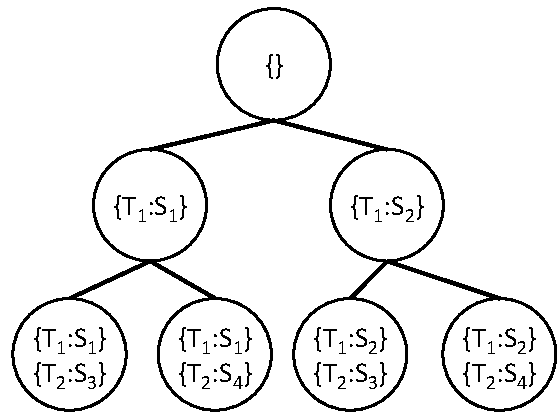
\includegraphics[width=0.6\columnwidth]{search-space-samd_cropped.pdf}
    \caption{An example of part of the \samd search space.}
    \label{fig:search-space}
\end{figure}

A graph search problem is defined by a graph $(V,E)$,
a node $s\in V$, and a set of nodes $G\subseteq V$,
where a solution is a path in the graph from $s$ to a node in $G$.
The graph can be explicitly given as input, or implicitly given
by defining an initial node and a set of transition functions
that map a node to its neighbors in the graph.

\samd can be represented as a search problem in the following graph. A node in the graph represents a \emph{partial} supplier assignment function,
which is function that assigns suppliers to a subset of the tasks in $T$.
The initial node $s$ is the empty supplier assignment function, that is, a partial supplier assignment function that does not assign any supplier to any tasks.
Every child node of $s$ represents a possible assignment of a supplier to $T_1$.
Every child node of these nodes represents a possible assignment of a supplier to $T_2$,
and so forth. Note that this search space is a tree. Figure~\ref{fig:search-space} illustrates two levels of this tree.
The depth of this tree is the number of tasks $N$, and every leaf node represents a \emph{complete} supplier assignment.


\subsection{A$^*$ for \samd}
\label{sec:astar}



\begin{algorithm}
\small
\KwIn{$\Pi=\tuple{T,S,X,d}$, an \samd problem}
\KwOut{$\varphi$, an optimal supplier assignment}
    $M_{best}\gets 0$; $\varphi_{best}\gets$ null; $\varphi_{init}=\{\}$; \open $\gets \emptyset$\\
    $n_{init}$.task$\gets 0$; $n_{init}$.$\varphi\gets \varphi_{init}$\\
    Add $n_{init}$ to \open with key $U(n_{init})$\\
    \While{\open is not empty}{
        $n_{best}\gets$ pop from \open a node with maximal $U(n)$\\
        \If{$U(n_{best})\leq M_{best}$}{
            \Return $\varphi_{best}$\\
        }
        $i\gets n_{best}$.task\\
        $\varphi\gets n_{best}.\varphi$\\
        \ForEach{supplier $s$ for task $T_{i+1}$}{
            $n_{child}$.task $\gets i+1$\\    $n_{child}.\varphi\gets\varphi\cup(T_i\rightarrow s)$\\
            \eIf{$n_{child}.\varphi$ is a complete assignment}{
                $M\gets M(n_{child})$\\
                \If{$M\geq M_{best}$}{
                    $M_{best}\gets M$\\
                    $\varphi_{best}\gets n_{child}.\varphi$\\
                }
            }{
                Add $n_{child}$ to \open with key $U(n_{child})$\\
            }
        }
    }
    \Return $\varphi_{best}$\\
    \caption{Psuedo-code of \astar for \samd.}
	\label{alg:astar}
\end{algorithm}


To search this search space for the supplier assignment $\varphi$ that maximizes $M(T, \varphi, d)$,
we use the \astar algorithm~\cite{hart1968formal} with some adjustments.
\astar is a best-first search algorithm that maintains two lists of nodes: an open list (denoted \open) that contains all nodes that were generated and not expanded yet, and a closed list (denoted \closed) that contains all nodes that were already expanded. Initially, \open contains the initial node (in our case, the node representing an empty supplier assignment). Then, in every iteration one node is moved from \open to \closed, and all its children nodes are added to \open. The search halts when a goal node is popped from \open.

\astar considers two values for every node $n$:
the cost of the best-known path from the initial node to $n$,
and a heuristic estimate of the cost of the optimal path from a given node to a goal.
The former is denoted by $g(n)$ and the latter by $h(n)$. \astar pops from \open in every iteration the
node with the smallest $g(n)+h(n)$.
A heuristic $h$ is called \emph{admissible} if its estimate is never larger than the real cost of the optimal path from $n$ to the goal.
Given an admissible heuristic, \astar is guaranteed to have found the optimal solution when a goal node is expanded. Moreover, under certain conditions, all other algorithms must expand at least the same set of nodes as \astar~\cite{dechter1985generalized,holte2019OnThe}.


\astar is commonly used for minimization problems, but ~\cite{stern2014max} pointed out how to adapt it to solve maximization problems. Two changes are required: (1) for a heuristic function to be admissible it must return an estimate that is never \emph{smaller than} the real cost to reach a goal,
and (2) the search can only halt after the cost of the best solution found so far
is smaller than or equal to $g(n)+h(n)$ for all $n$ in \open.

To apply \astar as is to solve \samd, we need to define $g(n)$ and $h(n)$. However,
the notion of paths and costs of paths is not natural in our search space,
since we can only compute the actual value -- $M(T, \varphi,d)$ -- of a complete supplier assignment.
Instead of defining $g(n)$ and $h(n)$, we define for every node $n$ a single value, denoted $U(n)$,
that is an upper bound over the cost of all goal nodes in the subtree of the search space rooted by $n$.
Then, in every iteration of our modified \astar, we pop from \open the node with the highest $U(n)$ value
and insert its children to \open.
A leaf node represents a complete supplier assignment. So, for every generated leaf node $n$ we compute its corresponding $M$ value, and store the leaf with the highest $M$ seen so far. We refer to this leaf node as $n_{best}$ and its $M$ value as $M_{best}$.  The search halts when either \open is empty or the expanded node $n$ is such that $U(n)\leq M_{best}$. When the former condition occurs, we know that all supplier assignments have been checked, in which case $n_{best}$ is indeed optimal. If the latter condition occurs, we know that for all nodes $n\in \open$ it holds that $U(n)\leq M_{best}$, and thus $n_{best}$ is optimal. Consequently, given that an admissible $U(\cdot)$ is implemented, completeness and optimality are guaranteed~\cite{stern2014max,holte2019OnThe}.

Algorithm~\ref{alg:astar} provides a complete pseudo-code for our \astar-based algorithm. For convenience, for a node $n$ we denote by $n.\varphi$ and $n$.task
the partial assignment that $n$ represents and the index of the last task assigned by $n.\varphi$, respectively. Hence, for the initial node $n_{init}$ we have that $n_{init}.\varphi$ is an empty supplier assignment and $n_{init}.$task is zero (line 2 in Algorithm~\ref{alg:astar}). Note that due to the tree structure of the search graph, there is no need to maintain \closed.


\subsection{Computing an Upper Bound}

Our \astar can be used with any implementation of $U(\cdot)$ as long as it is admissible for maximization problems, i.e., returns a valid upper bound over all the goals in its sub-tree. Next, we propose a concrete admissible $U(\cdot)$ that works well in practice.

Let $n$ be the node we wish to compute $U(n)$ for, and assume that $n$ represents a partial assignment $\varphi_n$ that assigns a supplier to tasks $t_1,\ldots t_i$ for some $i<N$.
We compute $U(n)$ by assuming that in every unassigned task $t\in \{t_{i+1},\ldots,t_{N}\}$
all suppliers that can perform this task do so simultaneously, so that the task is completed
when the fastest one finished. Formally, for the computation of $U(n)$, we assume that the completion time of every unassigned task $t$ to be $\min_{s\in S_t} X_s$. This is a random variable that can be computed easily given all the $X_s$ random variables. Since in our setting only a single supplier performs each task, the real completion time of any single supplier must be larger than this value (or at least equal). Thus, it can be used as an admissible heuristic.

To summarize, we define $U(n)$ as follows:
\begin{equation}
U(n)=\sum_{t\in \{t_1,\ldots t_i\}} X_{\varphi_n(t)} + \sum_{t\in \{t_{i+1},\ldots t_{N}\}} \min_{s\in S_t} X_s
\label{eq:heuristic}
\end{equation}




While the above $U(\cdot)$ is clearly admissible, its computational effort is equivalent to that of the $M(T,\varphi,d)$ value of some complete supplier assignment $\varphi$, which is NP-hard (Corollary~\ref{cor:m}). For small problems it may be feasible to apply such a computation for a limited number of times, as is done in \sampling. However, $U(n)$ needs to be computed frequently for every node $n$ that is added to \open, which renders its exact computation inapplicable. Hence, we turn to an approximate computation of $U(\cdot)$.

Recall that the problem with computing the $M$ value lies in the exponential growth of the support size \cite{cohen2015estimating}. Consequently, after every addend in the computation of $U(\cdot)$ we apply the \optapprox$(X,m)$ operator \cite{cohen2018optimal}, which for a given random variable $X$ and a requested support size $m$ returns a new random variable $X'$ with a support size of at most $m$ in polynomial time. By restricting the support size to a given $m$ after every addend, we prevent the exponential growth of the support size.

The resulting $X'$ of \optapprox$(X,m)$ is actually the best approximation (optimal) of $X$ given the requested support size $m$ according to the ``one-sided'' version of the Kolmogorov distance. The ``one-sided'' approximation means that the \emph{cumulative distribution function} (CDF) $F_{X'}$ of $X'$ is greater or equal to the CDF $F_{X}$ of $X$, i.e., for every value $v$ of $X$, $F_{X}(v)\leq F_{X'}(v)$. This, in turn, results in a pessimistic computation of the probability to meet the deadline. Consequently, we use an inverse version of \optapprox that gives $F_{X}(v)\geq F_{X'}(v)$ for all $v$, i.e., an optimistic computation of the probability to meet the deadline. We term the computation of $U(\cdot)$ with the inverse version of \optapprox after every addend as $U_{\optapprox}(\cdot)$.

\begin{lemma}
$U_{\optapprox}(\cdot)$ is admissible.
\label{lem:admissible}
\end{lemma}

\begin{proof}
$U(\cdot)$ is trivially admissible, since it assumes that all suppliers that can perform a future task will do so simultaneously, which is obviously not worse than any single supplier performing the task. Also, the inverse version of \optapprox that is applied in $U_{\optapprox}(\cdot)$ is optimistic, hence also admissible.
\end{proof}

\begin{corollary}
\astar for \samd is complete and optimal.
\end{corollary}

Note that in order to maintain the optimality of the algorithm we cannot use \optapprox in the computation of $M$ for complete supplier assignments (line 14 in Algorithm~\ref{alg:astar}). Theoretically, this computation is performed an exponential number of times. Nonetheless, in practice our \astar approach manages to refrain from expanding most of the leaves (complete assignments), as is evident from the run-time results of our experimental evaluation (Section~\ref{sec:exp}).




\section{Experimental Evaluation}
\label{sec:exp}

In what follows we experimentally evaluate the performance of four algorithms -- two sub-optimal algorithms, \sampling with 100 samples (Subsection~\ref{sec:sampling}) and \expectation (Subsection~\ref{sec:expect}), and two optimal algorithms, the \astar-based algorithm (Subsection~\ref{sec:astar}) and the brute-force approach that was presented at the beginning of Section~\ref{sec:opt}.
We compare between the four algorithms in terms of run-time performance and solution quality. For evaluating the solution quality of the sub-optimal methods we use two measures -- the average error, i.e., the difference from the optimal probability to meet a deadline, and the percentage of instances in which the optimal solution is found. Obviously, the optimal approaches have no error and always find the optimal solution.

We consider various experimental setups of both synthetically-generated completion-time distributions and distributions extracted from real software projects. The problem instances are in the form of a graph with different number of layers (tasks) and different number of nodes in each layer (suppliers). We also compare three deadline types that are derived from $maxd$, where $maxd$ is the maximal possible completion time of a project given the maximal values of the distributions of the suppliers (excluding the value of failure, Subsection~\ref{sec:SynthericDist}) and the number of tasks. The deadline types are early ($0.25\cdot maxd$), expected ($0.5\cdot maxd$), and late ($0.75\cdot maxd$). We use various deadlines in order to examine their effect on the different algorithms, especially on \expectation. Intuitively, we presume that \expectation will perform well for expected deadlines.

\subsection{Synthetic Distributions}
\label{sec:SynthericDist}
We consider three types of synthetically generated distributions -- random, structural, and structural with failure. We use a support size of 4 in all the distributions. In the \emph{random distribution} we generate possible completion times for each supplier in the range [0\dots 4] with uniform distribution. The distribution is also randomly generated and then normalized to sum up to one. An example of a random distribution may look like [0.58:0.23, 3.24:0.32, 3.87:0.17, 3.44:0.28].
In the \emph{structural distribution} we uniformly generate a single possible completion time between every two consecutive integers, and the distribution is generated as in the random distribution. An example of a structural distribution may look like [0.58:0.15, 1.24:0.59, 2.87:0.01, 3.44:0.25]. In the \emph{structural with failure distribution} we generate the possible completion times as in the structural distribution, except for the last value that is always set to $10^6$. This large value represents in practice a situation in which the supplier can never complete the task, or in other words -- fail. Indeed, in real-world situations, some suppliers may fail at performing a task. An example of structural with failure distribution (or failure for short) may look like [0.58:0.14, 1.24:0.41, 2.87:0.33, $10^6$:0.12].
Note that in our experiments we do not consider normal distributions, since such problems are much easily solvable, as the sum of normal distribution can be computed in polynomial time~\cite{schattenberg2005project,glaubius2009scheduling,olya2014applying}.


We vary the number of tasks (layers) in a project. Due to the obvious limitations of the exponential search space, we used a 10 minute time-out for each instance, which was sufficient to run up to 8 layers with the brute-force approach. For every setting composed of the number of layers, the distribution type, and the deadline duration, we run 30 different problem instances in order to gather significant statistics. For every task we consider two possible suppliers, each with a different distribution. In addition, we use a support size of 4, since the brute-force approach failed to solve problems with larger support size due to lack of memory.

\subsection{Distributions from Software Development}
The next type of distributions we use is aimed to simulate a \samd problem of a software project, in which the suppliers are software developers and the tasks are \emph{user stories} that need to be implemented by a developer. A user story in software development is ``a small piece of functionality of the final software perceived from the end-user point of view''~\cite{rees2002feasible},
and is one of the most common ways to specify requirements~\cite{kassab2015changing}. We extracted information about implemented user stories from three open-source projects: (1) JBoss Developer,\footnote{\url{https://issues.jboss.org}} (2) Lsst DM,\footnote{\url{https://jira.lsstcorp.org}} and (3) Spring XD.\footnote{\url{https://jira.spring.io}}
Specifically, we extracted the list of user stories that were assigned to a developer and marked as done. For each user story, we extracted the developer assigned to implement it and the number of \emph{sprints} it took to implement this user story. A sprint corresponds to a fixed time frame, which is either two or three weeks in most projects. Using this data, we created for every developer a distribution of the number of sprints that developer needs to implement a user story. In total we obtained the distributions of user story completion time for 39 developers. Here is examples for a developers distributions [1:0.95,	2:0.045, 3:0.005] or [1:0.62,	2:0.3,	3:0.07,	4:0.01].
We note that this information is publicly available from JIRA, a popular issue tracking system used by all our projects to manage the development. See the footnotes above for links to this publicly available data.


With these distributions, we generate three types of SAMD problems as follows. The first has four tasks (Developer, DM1, DM2, XD), with each task having all the possible developers from that task's developer pool. This project is unique, and we examine the probability to meed the deadline for different deadlines, up to 20 sprints. The second type is of randomly generated projects with 4 tasks (Developer, DM1, DM2, XD), where for each task we randomly select (without repetitions) developers from the relevant developer pool. We examine how the different number of suppliers in each task (up to 7 suppliers) affects the run-time and solution quality.
In the third type the number of developers is set to 4 for every task, i.e., we randomly select (without repetitions) 4 developers from the relevant developer pool. The parameter we vary here is the number of layers, up to 7 layers. We randomly generate 30 instances for each of the latter two problem types.


\subsection{Results}
\label{sec:res}

We start with presenting the results for the experiments with synthetic distributions. Note that since the \astar algorithm and the brute-force approach are both optimal, their error is always zero and thus we do not present their error results.

Figure~\ref{025rt} compares the run-times of the four algorithms.
In all conducted experiments (in all of the settings) the run-time of the \astar algorithm outperforms that of the brute-force algorithm. In addition, one can also see that the run-time of \astar is smaller than the run-time of \sampling, which is not optimal in most cases. In all experiments, the run-time of the \expectation heuristic algorithm is considerably shorter than all other approaches, however its solution quality is low and in some cases even returns an error of 1.
In other words, the \astar algorithm guarantees optimality in reasonable run-time. \expectation and \sampling heuristic algorithms result with an error and do not return the optimal assignment.
For instance, the error comparison results for 6 layers (of the experiment in Figure~\ref{025rt}) shows that an error of $1.6\cdot 10^{-5}$ for \expectation and $0.006$ for \sampling. For 7 layers the respective errors are $7 \cdot 10^{-5}$ and $0.004$, and for 8 layers they are $4 \cdot 10^{-5}$ and $0.003$. %Although we can see that \expectation run-time is negligible (less than one second), it produces error.  [[Roni: meaningless sentence]]

\begin{figure}[h!]
	\scriptsize
	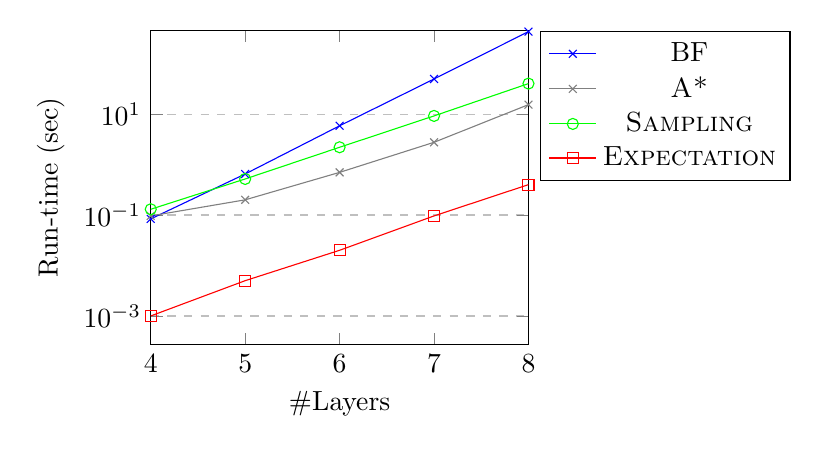
\begin{tikzpicture}
	\begin{axis}[
	scale=0.7,
	ymode=log,
	xlabel={\#Layers},
	ylabel near ticks,
	ylabel={Run-time (sec)},
	xmin=4, xmax=8,
	ymin=0, ymax=450,
	legend pos=outer north east,
	ymajorgrids=true,
	grid style=dashed,
	]

	\addplot[
	color=blue,
	mark=x,
	]
	coordinates {
		(4 , 0.0837)
		(5 , 0.65)
		(6 , 5.86)
		(7 , 49.6)
		(8 , 431.27)

	};
	\addlegendentry{BF}

	\addplot[
	color=gray,
	mark=x,
	]
	coordinates {
		(4 , 0.096)
		(5 , 0.2)
		(6 , 0.7)
		(7 , 2.76)
		(8 , 15.38)

	};
	\addlegendentry{\astar}

	\addplot[
	color=green,
	mark=o,
	]
	coordinates {
		(4 , 0.13)
		(5 , 0.518)
		(6 , 2.2)
		(7 , 9.2)
		(8, 40.2)

	};
	\addlegendentry{\sampling}

	\addplot[
	color=red,
	mark=square,
	]
	coordinates {
		(4 , 0.001)
		(5 , 0.005)
		(6 , 0.02)
		(7 , 0.096)
		(8, 0.4)

	};
	\addlegendentry{\expectation}

	\end{axis}
	\end{tikzpicture}
	\caption{Run-time comparison of all algorithms for deadline of size $0.25\cdot maxd$ and random distribution}\label{025rt}
\end{figure}

\begin{comment}

\begin{figure}[h!]
	\scriptsize
	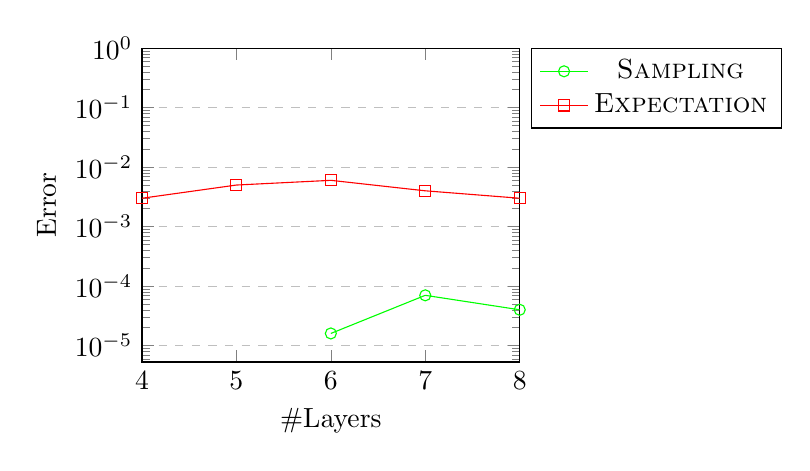
\begin{tikzpicture}
	\begin{axis}[
	scale=0.7,
	ymode=log,
	xlabel={\#Layers},
	ylabel near ticks,
	ylabel={Error},
	xmin=4, xmax=8,
	ymin=0, ymax=1,
	legend pos=outer north east,
	ymajorgrids=true,
	grid style=dashed,
	]

		\addplot[
	color=green,
	mark=o,
	]
	coordinates {
		(4 , 0)
		(5 , 0)
		(6 , 0.000016)
		(7 , 0.00007)
		(8 , 0.00004)

	};
	\addlegendentry{\sampling}

	\addplot[
	color=red,
	mark=square,
	]
	coordinates {
		(4 , 0.003)
		(5 , 0.005)
		(6 , 0.006)
		(7 , 0.004)
		(8, 0.003)

	};
	\addlegendentry{\expectation}

	\end{axis}
	\end{tikzpicture}
	\caption{Error comparison of all heuristic algorithms for deadline of size $0.25\cdot maxd$ and random distribution}\label{025rand}
\end{figure}

\end{comment}


It is interesting to illuminate the fact that the \expectation heuristic can not handle correctly some types of distributions.
\begin{example}
Let us observe the following Failure distribution [1:0.99, $10^6$:0.01] and the following uniform distribution [100:0.5, 200:0.5]. For every task, assume two suppliers, one supplier has the uniform duration distribution (call it $u$), and the other supplier has the Failure duration distribution (call it $f$). For a project with two tasks and a deadline of 10 seconds, the \expectation heuristic algorithm will choose for both tasks supplier $u$ because its expectation is smaller. Eventually the \expectation heuristic algorithm returns zero chance to meet the deadline where in fact there is a chance of almost 100\% to succeed.
\end{example}
The errors we get when using the \expectation heuristic algorithm in our experiments with Failure distribution are 0.51-0.7, depending on the number of layers; note that such errors are high (the range is 0-1). We witness such high errors because the \expectation heuristic algorithm returns that there is no chance to meet the deadline where in fact there is. The other algorithms executed in a setting with this Failure distribution resulted with an error equal to 0. In addition, for all other approaches we got 97\%-100\% correct optimal assignment for every number of layers, but using the \expectation heuristic algorithm we did not get any right assignment for any number of layers.


\commentout{
\begin{figure}[h!]
	\scriptsize
	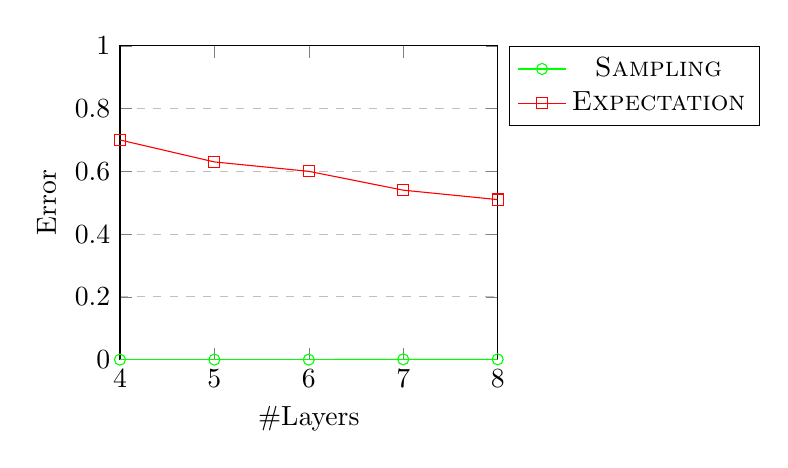
\begin{tikzpicture}
	\begin{axis}[
	scale=0.7,
	xlabel={\#Layers},
	ylabel near ticks,
	ylabel={Error},
	xmin=4, xmax=8,
	ymin=0, ymax=1,
	legend pos=outer north east,
	ymajorgrids=true,
	grid style=dashed,
	]

	\addplot[
	color=green,
	mark=o,
	]
	coordinates {
		(4 , 0)
		(5 , 0)
		(6 , 0)
		(7 , 0.001)
		(8 , 0.001)

	};
	\addlegendentry{\sampling}

    \addplot[
	color=red,
	mark=square,
	]
	coordinates {
		(4 , 0.7)
		(5 , 0.63)
		(6 , 0.6)
		(7 , 0.54)
		(8 , 0.51)

	};
	\addlegendentry{\expectation}

	\end{axis}
	\end{tikzpicture}
	\caption{Error comparison of all heuristic algorithms for deadline of size $0.75\cdot maxd$ and ``Failure" distribution}\label{075faile}
\end{figure}
}
\commentout{
\begin{figure}[h!]
	\scriptsize
	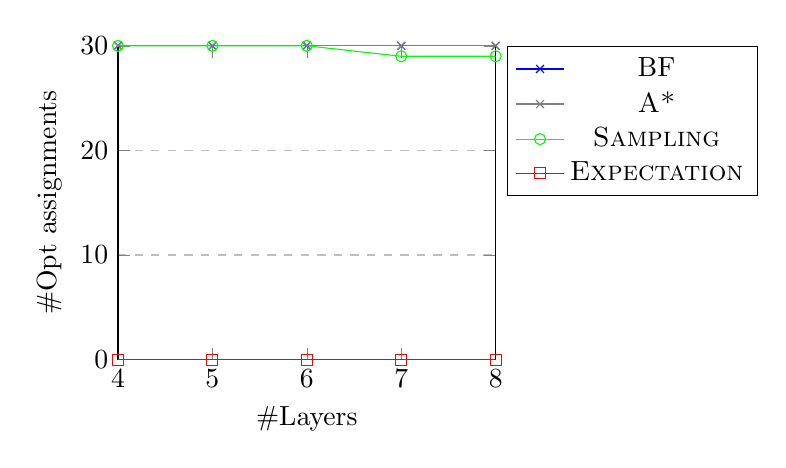
\begin{tikzpicture}
	\begin{axis}[
	scale=0.7,
	xlabel={\#Layers},
	ylabel near ticks,
	ylabel={\#Opt assignments},
	xmin=4, xmax=8,
	ymin=0, ymax=30,
	legend pos=outer north east,
	ymajorgrids=true,
	grid style=dashed,
	]

	\addplot[
	color=blue,
	mark=x,
	]
	coordinates {
		(4 , 30)
		(5 , 30)
		(6 , 30)
		(7 , 30)
		(8 , 30)

	};
	\addlegendentry{BF}

	\addplot[
	color=gray,
	mark=x,
	]
	coordinates {
		(4 , 30)
		(5 , 30)
		(6 , 30)
		(7 , 30)
		(8 , 30)

	};
	\addlegendentry{\astar}

	\addplot[
	color=green,
	mark=o,
	]
	coordinates {
		(4 , 30)
		(5 , 30)
		(6 , 30)
		(7 , 29)
		(8 , 29)

	};
	\addlegendentry{\sampling}

	\addplot[
	color=red,
	mark=square,
	]
	coordinates {
		(4 , 0)
		(5 , 0)
		(6 , 0)
		(7 , 0)
		(8 , 0)

	};
	\addlegendentry{\expectation}

	\end{axis}
	\end{tikzpicture}
	\caption{Number of optimal assignments comparison of all heuristic algorithms for deadline of size $0.75\cdot maxd$ and ``Failure" distribution}\label{075failn}
\end{figure}
}

Another concern regarding the \expectation heuristic is the chosen deadline. As long as the deadline is around the average duration, it is more likely that the \expectation heuristic algorithm will return solid results. However, the deadline is not strict, and in the general case, where the deadline can be very small or very large compared to the expectation, this heuristic may produce substantially sub-optimal results. For a deadline such as $0.5\cdot maxd$ we can observe good results produced by the \expectation heuristic algorithm due to the comfortable deadline. For 4, 5, 6, 7, 8 layers the results are 93\%, 80\%, 70\%, 90\%, 90\% optimal assignments, respectively.

\commentout{
\begin{figure}[h!]
	\scriptsize
	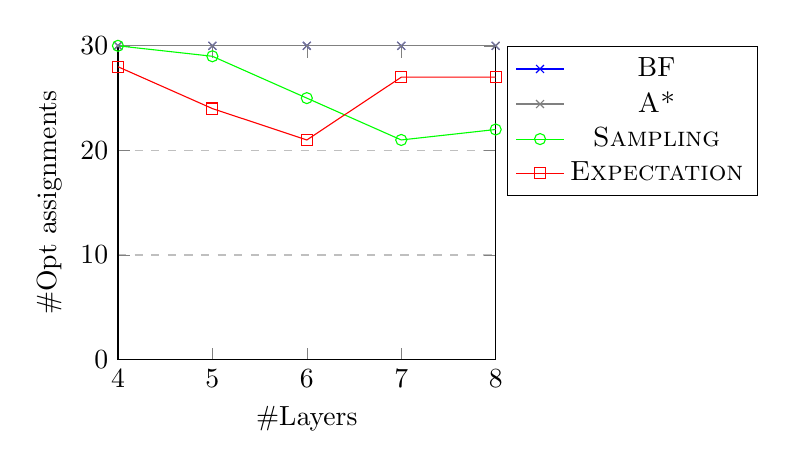
\begin{tikzpicture}
	\begin{axis}[
	scale=0.7,
	xlabel={\#Layers},
	ylabel near ticks,
	ylabel={\#Opt assignments},
	xmin=4, xmax=8,
	ymin=0, ymax=30,
	legend pos=outer north east,
	ymajorgrids=true,
	grid style=dashed,
	]

	\addplot[
	color=blue,
	mark=x,
	]
	coordinates {
		(4 , 30)
		(5 , 30)
		(6 , 30)
		(7 , 30)
		(8 , 30)

	};
	\addlegendentry{BF}

	\addplot[
	color=gray,
	mark=x,
	]
	coordinates {
		(4 , 30)
		(5 , 30)
		(6 , 30)
		(7 , 30)
		(8 , 30)

	};
	\addlegendentry{\astar}

	\addplot[
	color=green,
	mark=o,
	]
	coordinates {
		(4 , 30)
		(5 , 29)
		(6 , 25)
		(7 , 21)
        (8 , 22)
	};
	\addlegendentry{\sampling}


	\addplot[
	color=red,
	mark=square,
	]
	coordinates {
		(4 , 28)
		(5 , 24)
		(6 , 21)
		(7 , 27)
		(8 , 27)

	};
	\addlegendentry{\expectation}



	\end{axis}
	\end{tikzpicture}
	\caption{Number of optimal assignments comparison of all heuristic algorithms for deadline of size $0.5\cdot maxd$ and ``Structural" distribution}\label{05reg}
\end{figure}}

As the number of layers grows, the \sampling heuristic is less accurate. Even though, the error is somewhat small, the number of optimal assignments is reducing as a function of the number of layers, see Table~\ref{tableOptAssgn}. Since the number of possible assignments is growing (exponentially) as the number of layers grows, the \sampling heuristic needs more samples in order to return good solution, which increases run-time. Here we used 100 samples for each experiment.

\begin{table}[]
\centering
\small
\begin{tabular}{|l|l|l|l|l|l|l|}
\hline
\multirow{2}{*}{\textbf{Deadl.}} & \multirow{2}{*}{\textbf{Alg.}} & \multicolumn{5}{c|}{\textbf{\#Layers}}                         \\ \cline{3-7}
                                   &                                     & \textbf{4} & \textbf{5} & \textbf{6} & \textbf{7} & \textbf{8} \\ \hline
\multirow{3}{*}{$0.75$}  & \astar/BF                                  & 100\%         & 100\%         & 100\%         & 100\%         & 100\%         \\ \cline{2-7}
                                   & Sampl.                            & 93\%         & 97\%         & 87\%         & 70\%         & 47\%         \\ \cline{2-7}
                                   & Exp.                         & 57\%         & 57\%         & 50\%         & 30\%          & 17\%          \\ \hline
\multirow{3}{*}{$0.25$}  & \astar/BF                                  & 100         & 100\%         & 100\%         & 100\%         & 100\%         \\ \cline{2-7}
                                   & Sampl.                            & 97\%         & 100\%         & 83\%         & 77\%         & 57\%         \\ \cline{2-7}
                                   & Exp.                         & 33\%         & 30\%          & 27\%          & 33\%         & 10\%          \\ \hline
\end{tabular}
\caption{Number of optimal assignments comparison (in percentage out of 30) of all algorithms for deadline of size $0.75\cdot maxd$ and $0.25\cdot maxd$ with structural distribution}\label{tableOptAssgn}
\end{table}


\commentout{
\begin{figure}[h!]
	\scriptsize
	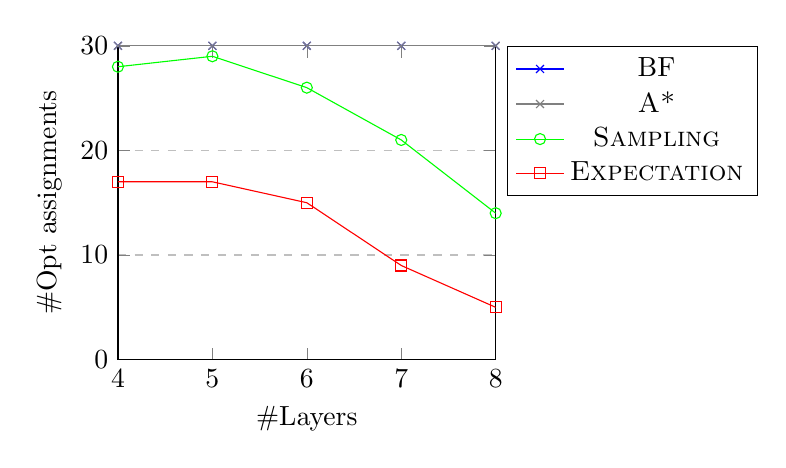
\begin{tikzpicture}
	\begin{axis}[
	scale=0.7,
	xlabel={\#Layers},
	ylabel near ticks,
	ylabel={\#Opt assignments},
	xmin=4, xmax=8,
	ymin=0, ymax=30,
	legend pos=outer north east,
	ymajorgrids=true,
	grid style=dashed,
	]

	\addplot[
	color=blue,
	mark=x,
	]
	coordinates {
		(4 , 30)
		(5 , 30)
		(6 , 30)
		(7 , 30)
		(8 , 30)

	};
	\addlegendentry{BF}

	\addplot[
	color=gray,
	mark=x,
	]
	coordinates {
		(4 , 30)
		(5 , 30)
		(6 , 30)
		(7 , 30)
		(8 , 30)

	};
	\addlegendentry{\astar}

	\addplot[
	color=green,
	mark=o,
	]
	coordinates {
		(4 , 28)
		(5 , 29)
		(6 , 26)
		(7 , 21)
		(8 , 14)

	};
	\addlegendentry{\sampling}

	\addplot[
	color=red,
	mark=square,
	]
	coordinates {
		(4 , 17)
		(5 , 17)
		(6 , 15)
		(7 , 9)
        (8 , 5)
	};
	\addlegendentry{\expectation}



	\end{axis}
	\end{tikzpicture}
	\caption{Number of optimal assignments comparison of all heuristic algorithms for deadline of size $0.75\cdot maxd$ and ``Structural" distribution}\label{075regn}
\end{figure}

\begin{figure}[h!]
	\scriptsize
	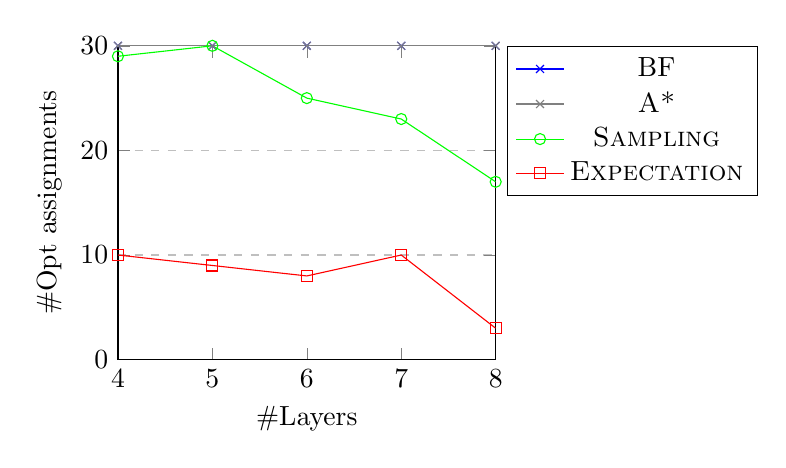
\begin{tikzpicture}
	\begin{axis}[
	scale=0.7,
	xlabel={\#Layers},
	ylabel near ticks,
	ylabel={\#Opt assignments},
	xmin=4, xmax=8,
	ymin=0, ymax=30,
	legend pos=outer north east,
	ymajorgrids=true,
	grid style=dashed,
	]

	\addplot[
	color=blue,
	mark=x,
	]
	coordinates {
		(4 , 30)
		(5 , 30)
		(6 , 30)
		(7 , 30)
		(8 , 30)

	};
	\addlegendentry{BF}

	\addplot[
	color=gray,
	mark=x,
	]
	coordinates {
		(4 , 30)
		(5 , 30)
		(6 , 30)
		(7 , 30)
		(8 , 30)

	};
	\addlegendentry{\astar}

	\addplot[
	color=green,
	mark=o,
	]
	coordinates {
		(4 , 29)
		(5 , 30)
		(6 , 25)
		(7 , 23)
		(8 , 17)

	};
	\addlegendentry{\sampling}


	\addplot[
	color=red,
	mark=square,
	]
	coordinates {
		(4 , 10)
		(5 , 9)
		(6 , 8)
		(7 , 10)
		(8 , 3)

	};
	\addlegendentry{\expectation}


	\end{axis}
	\end{tikzpicture}
	\caption{Number of optimal assignments comparison of all heuristic algorithms for deadline of size $0.25\cdot maxd$ and ``Structural" distribution}\label{025regn}
\end{figure}


\begin{figure}
	\scriptsize
	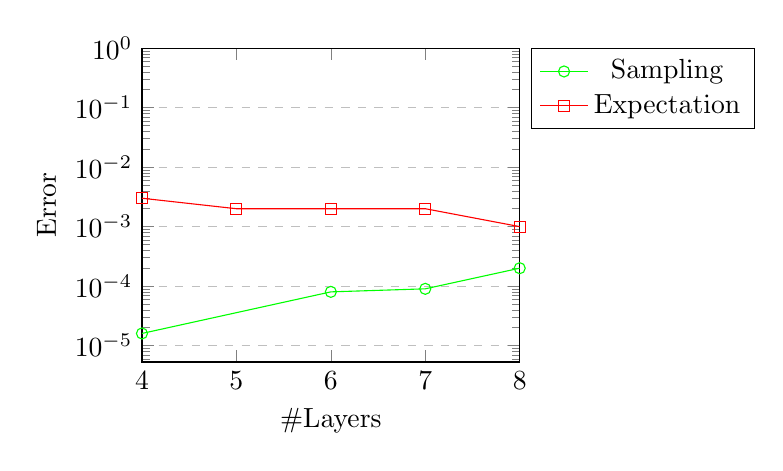
\begin{tikzpicture}
	\begin{axis}[
	scale=0.7,
	ymode = log,
	xlabel={\#Layers},
	ylabel near ticks,
	ylabel={Error},
	xmin=4, xmax=8,
	ymin=0, ymax=1,
	legend pos=outer north east,
	ymajorgrids=true,
	grid style=dashed,
	]

	\addplot[
	color=green,
	mark=o,
	]
	coordinates {
		(4 , 0.000016)
		(5 , 0)
		(6 , 0.00008)
		(7 , 0.00009)
		(8 , 0.0002)

	};
	\addlegendentry{Sampling}

	\addplot[
	color=red,
	mark=square,
	]
	coordinates {
		(4 , 0.003)
		(5 , 0.002)
		(6 , 0.002)
		(7 , 0.002)
		(8 , 0.001)

	};
	\addlegendentry{Expectation}



	\end{axis}
	\end{tikzpicture}
	\caption{Error comparison of all heuristic algorithms for deadline of size $0.25\cdot maxd$ and Structural distribution}\label{025rege}
\end{figure}

\begin{figure}[h!]
	\scriptsize
	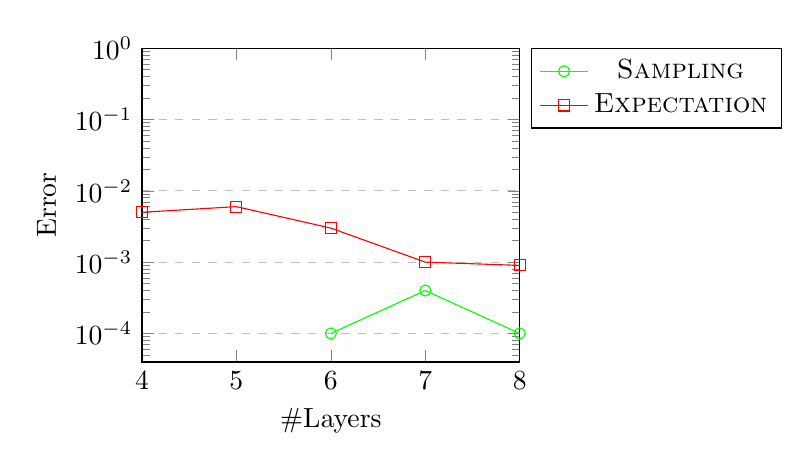
\begin{tikzpicture}
	\begin{axis}[
	scale=0.7,
	ymode=log,
	xlabel={\#Layers},
	ylabel near ticks,
	ylabel={Error},
	xmin=4, xmax=8,
	ymin=0, ymax=1,
	legend pos=outer north east,
	ymajorgrids=true,
	grid style=dashed,
	]

	\addplot[
	color=green,
	mark=o,
	]
	coordinates {
		(4 , 0)
		(5 , 0)
		(6 , 0.0001)
		(7 , 0.0004)
        (8 , 0.0001)
	};
	\addlegendentry{\sampling}

	\addplot[
	color=red,
	mark=square,
	]
	coordinates {
		(4 , 0.005)
		(5 , 0.006)
		(6 , 0.003)
		(7 , 0.001)
        (8 , 0.0009)
	};
	\addlegendentry{\expectation}



	\end{axis}
	\end{tikzpicture}
	\caption{Error comparison of all heuristic algorithms for deadline of size $0.75\cdot maxd$ and random distribution}\label{075rande}
\end{figure}
}
The run-time plots are mostly similar, and as described before, the \astar heuristic algorithm presents the second best performance in aspect of run-time, see Figure~\ref{025rt}.
The best run-time is presented by \expectation heuristic algorithm, however, the solution quality of this method is poor.


\commentout{
\begin{figure}[h!]
	\scriptsize
	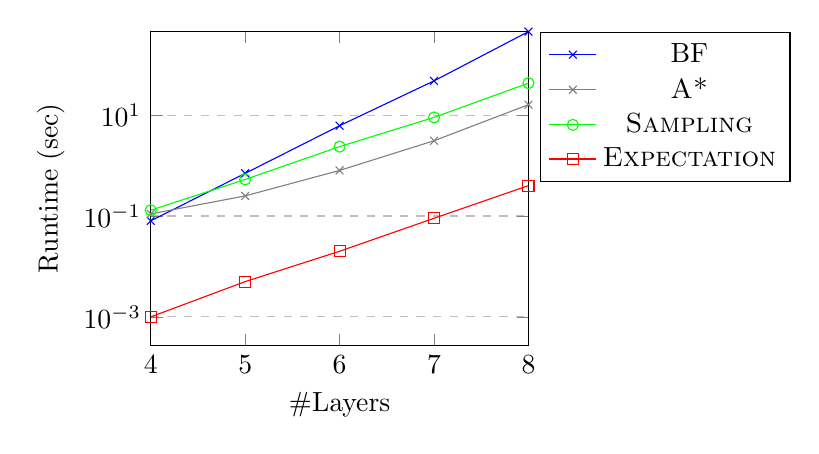
\begin{tikzpicture}
	\begin{axis}[
	scale=0.7,
	ymode = log,
	xlabel={\#Layers},
	ylabel near ticks,
	ylabel={Runtime (sec)},
	xmin=4, xmax=8,
	ymin=0, ymax=452,
	legend pos=outer north east,
	ymajorgrids=true,
	grid style=dashed,
	]

	\addplot[
	color=blue,
	mark=x,
	]
	coordinates {
		(4 , 0.08)
		(5 , 0.7)
		(6 , 6.16)
		(7 , 47.67)
		(8 , 452)

	};
	\addlegendentry{BF}

	\addplot[
	color=gray,
	mark=x,
	]
	coordinates {
		(4 , 0.11)
		(5 , 0.25)
		(6 , 0.8)
		(7 , 3.1)
		(8 , 16.1)

	};
	\addlegendentry{\astar}


		\addplot[
	color=green,
	mark=o,
	]
	coordinates {
		(4 , 0.13)
		(5 , 0.53)
		(6 , 2.37)
		(7 , 9)
		(8 , 43)

	};
	\addlegendentry{\sampling}

	\addplot[
	color=red,
	mark=square,
	]
	coordinates {
		(4 , 0.001)
		(5 , 0.005)
		(6 , 0.02)
		(7 , 0.09)
		(8 , 0.4)

	};
	\addlegendentry{\expectation}

	\end{axis}
	\end{tikzpicture}
	\caption{Run time comparison of all heuristic algorithms for deadline of size $0.25\cdot maxd$ and ``Failure" distribution}\label{025failrt}
\end{figure}
}


Now we report the results of our experiments on the software development distribution types described earlier.
Figure~\ref{allDDRealError} shows how the deadline ($x$-axis) effects the error ($y$-axis).
As expected, for later deadlines the error is smaller, since many different assignments will meet the deadline with certainty. Also, for early deadlines where there in no chance to meet the deadline (omitted from the figure). For different deadlines, even on the same instance, the error may change dramatically. Contrary to that, the \astar algorithm is not sensitive for such deadline changes and always returns the optimal result.


\begin{figure}[h!]
	\scriptsize
	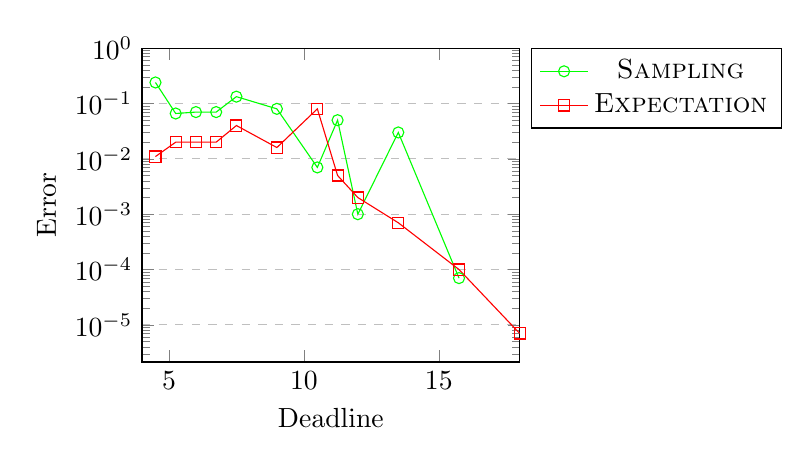
\begin{tikzpicture}
	\begin{axis}[
	scale=0.7,
	ymode = log,
	xlabel={Deadline},
	ylabel near ticks,
	ylabel={Error},
	xmin=4, xmax=18,
	ymin=0, ymax=1,
	legend pos=outer north east,
	ymajorgrids=true,
	grid style=dashed,
	]

	\addplot[
	color=green,
	mark=o,
	]
	coordinates {
		(0.75 , 0)
		(1.5 , 0)
		(3 , 0)
		(3.75 , 0)
		(4.5 , 0.24)
		(5.25 , 0.066)
		(6 , 0.07)
		(6.75 , 0.07)
		(7.5 , 0.133)
		(9 , 0.08)
		(10.5 , 0.007)
		(11.25 , 0.05)
		(12 , 0.001)
		(13.5 , 0.03)
		(15.75 , 0.00007)
		(18 , 0)
	};
	\addlegendentry{\sampling}

	\addplot[
	color=red,
	mark=square,
	]
	coordinates {
		(0.75 , 0)
		(1.5 , 0)
		(3 , 0)
		(3.75 , 0)
		(4.5 , 0.011)
		(5.25 , 0.02)
		(6 , 0.02)
		(6.75 , 0.02)
		(7.5 , 0.04)
		(9 , 0.016)
		(10.5 , 0.08)
		(11.25 , 0.005)
		(12 , 0.002)
		(13.5 , 0.0007)
		(15.75 , 0.0001)
		(18 , 0.000007)
	};
	\addlegendentry{\expectation}
	\end{axis}
	\end{tikzpicture}
	\caption{Error comparison of all algorithms for different deadlines and real data distribution}\label{allDDRealError}
\end{figure}

The next results we present are from the setting where the number of tasks is constant (4 tasks) and the number of possible suppliers to execute the task is changed. Here we can see how the error grows when we add more suppliers, mostly in the case of the \sampling heuristic algorithm. Similarly, the number of optimal assignments decreases as we add more optional suppliers, see Table~\ref{RealDataNoesDD4Error}. In this setting we increase the search space when we add more options for suppliers. The first heuristic to be affected by it is the \sampling heuristic algorithm. As the search space grows more samples are needed in order to maintain accuracy which also affects run time.
The run-time results %in Figure~\ref{RealDataNoesDD4rt}
for this setting continue the same trend as before, where the brute force algorithm takes the longest run-time and the \expectation heuristic algorithm takes the shortest time (with an error). In the middle of the run-time range are \sampling and \astar, where \astar is slightly better, taking shorter time.


\begin{table}[h!]
\centering
\resizebox{0.95\columnwidth}{!}{
\begin{tabular}{|l|l|l|l|l|l|l|}
\hline
\multirow{2}{*}{\textbf{}}                                                        & \multirow{2}{*}{\textbf{Alg.}} & \multicolumn{5}{c|}{\textbf{\#Suppliers}}                       \\ \cline{3-7}
                                                                                  &                                     & \textbf{3} & \textbf{4} & \textbf{5} & \textbf{6} & \textbf{7} \\ \hline
\multirow{3}{*}{Error}                                                            & \astar/BF                                  & 0          & 0          & 0          & 0          & 0          \\ \cline{2-7}

                                                                                  & Sampl.                          & 0.009      & 0.05       & 0.09       & 0.08       & 0.09       \\ \cline{2-7}
                                                                                  & Exp.                         & 0.009      & 0.008      & 0.008      & 0.008      & 0.01       \\ \hline
\multirow{3}{*}{\begin{tabular}[c]{@{}l@{}}\#Opt\end{tabular}} & \astar/BF                                  & 100\%         & 100\%         & 100\%         & 100\%         & 100\%         \\ \cline{2-7}
                           & Sampl.                            & 40\%         & 3\%          & 0\%          & 0\%          & 0\%          \\ \cline{2-7}
                                                                                  & Exp.                         & 30\%          & 30\%          & 23\%          & 20\%          & 13\%          \\ \hline
\end{tabular}
}
\caption{Error comparison and number of optimal assignments (in percentage out of 30) of all algorithms for different number of suppliers in each layer, deadline of 4 seconds and real data distribution}\label{RealDataNoesDD4Error}
\end{table}


\commentout{
\begin{figure}[h!]
	\scriptsize
	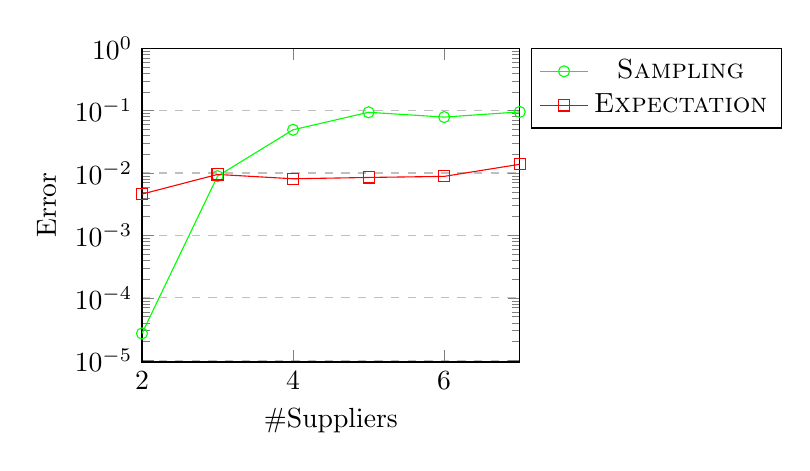
\begin{tikzpicture}
	\begin{axis}[
	scale=0.7,
	ymode = log,
	xlabel={\#Suppliers},
	ylabel near ticks,
	ylabel={Error},
	xmin=2, xmax=7,
	ymin=0, ymax=1,
	legend pos=outer north east,
	ymajorgrids=true,
	grid style=dashed,
	]



	\addplot[
	color=green,
	mark=o,
	]
	coordinates {
		(2 , 0.000027)
        (3,0.008913301)
        (4, 0.049329392)
        (5, 0.093992466)
        (6,0.078766868)
        (7,0.095318828)


	};
	\addlegendentry{\sampling}

	\addplot[
	color=red,
	mark=square,
	]
	coordinates {
		(2 , 0.0046023)
        (3,0.009501315)
        (4,0.008096098)
        (5,0.008501241)
        (6,0.008842637)
        (7,0.013824363)


	};
	\addlegendentry{\expectation}

	\end{axis}
	\end{tikzpicture}
	\caption{Error comparison of all heuristic algorithms for different number of suppliers in each layer, deadline of 4 seconds and real data distribution}\label{RealDataNoesDD4Error}
\end{figure}

\begin{figure}[h!]
	\scriptsize
	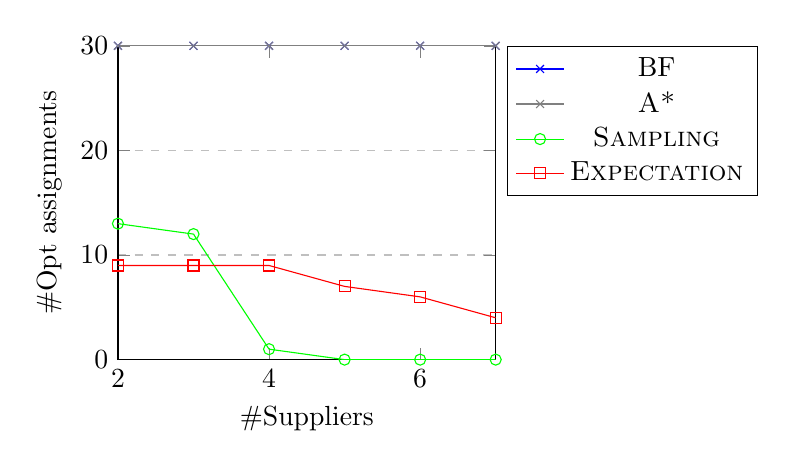
\begin{tikzpicture}
	\begin{axis}[
	scale=0.7,
	xlabel={\#Suppliers},
	ylabel near ticks,
	ylabel={\#Opt assignments},
	xmin=2, xmax=7,
	ymin=0, ymax=30,
	legend pos=outer north east,
	ymajorgrids=true,
	grid style=dashed,
	]

	\addplot[
	color=blue,
	mark=x,
	]
	coordinates {
		(2 , 30)
		(3 , 30)
		(4 , 30)
		(5 , 30)
		(6 , 30)
		(7 , 30)

	};
	\addlegendentry{BF}

	\addplot[
	color=gray,
	mark=x,
	]
	coordinates {
		(2 , 30)
		(3 , 30)
		(4 , 30)
		(5 , 30)
		(6 , 30)
		(7 , 30)

	};
	\addlegendentry{\astar}


		\addplot[
	color=green,
	mark=o,
	]
	coordinates {
		(2 , 13)
		(3 , 12)
		(4 , 1)
		(5 , 0)
		(6 , 0)
		(7 , 0)

	};
	\addlegendentry{\sampling}

	\addplot[
	color=red,
	mark=square,
	]
	coordinates {
		(2 , 9)
		(3 , 9)
		(4 , 9)
		(5 , 7)
		(6 , 6)
		(7 , 4)

	};
	\addlegendentry{\expectation}

	\end{axis}
	\end{tikzpicture}
	\caption{Number of optimal assignments comparison of all heuristic algorithms for different number of suppliers in each layer, deadline of 4 seconds and real data distribution}\label{RealDataNoesDD4Error}
\end{figure}
}

Finally, we vary the number of layers (tasks).
The error results are 0.04-0.06 for \sampling and 0.007-0.01 for \expectation. These algorithms detect only a few optimal assignments, \sampling less than 7\% and \expectation between 13\%-30\%, which is even less than what we already presented in similar experiment by using the synthetic distribution. In the real project distribution high probability goes with short time execution, we conjecture the results are affected by the shape of the probability.
\commentout{
\begin{figure}[h!]
	\scriptsize
	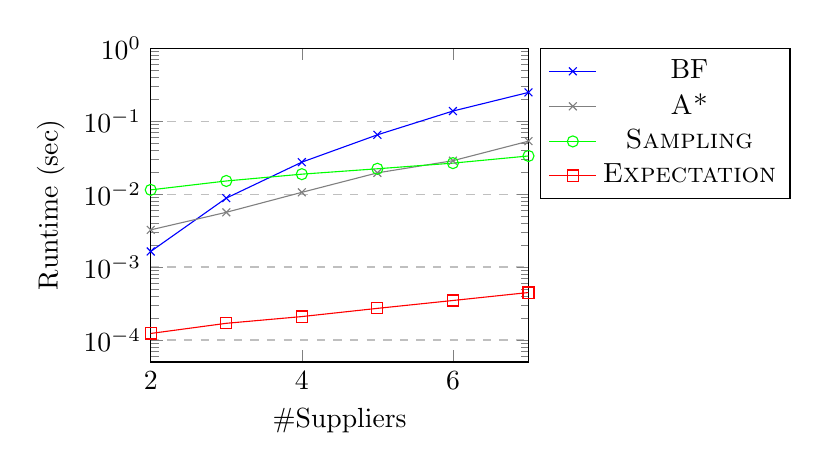
\begin{tikzpicture}
	\begin{axis}[
	scale=0.7,
	ymode = log,
	xlabel={\#Suppliers},
	ylabel near ticks,
	ylabel={Runtime (sec) },
	xmin=2, xmax=7,
	ymin=0, ymax=1,
	legend pos=outer north east,
	ymajorgrids=true,
	grid style=dashed,
	]

	\addplot[
	color=blue,
	mark=x,
	]
	coordinates {
		(2 , 0.001635782)
        (3, 0.008807731)
        (4,0.027389884)
        (5,0.064902401)
        (6,0.137466502)
        (7,0.24735659)
	};
	\addlegendentry{BF}

	\addplot[
	color=gray,
	mark=x,
	]
	coordinates {
		(2 , 0.00323391)
        (3,0.00562675)
        (4,0.010568492)
        (5,0.019532911)
        (6,0.028677018)
        (7,0.053106968)


	};
	\addlegendentry{\astar}


		\addplot[
	color=green,
	mark=o,
	]
	coordinates {
		(2 , 0.011423357)
        (3,0.015124575)
        (4,0.018751383)
        (5,0.022230466)
        (6,0.02655708)
        (7,0.033301409)


	};
	\addlegendentry{\sampling}

	\addplot[
	color=red,
	mark=square,
	]
	coordinates {
		(2 , 0.000122968)
        (3,0.000169365)
        (4,0.000209467)
        (5,0.000271455)
        (6,0.000347988)
        (7,0.000447472)
	};
	\addlegendentry{\expectation}

	\end{axis}
	\end{tikzpicture}
	\caption{Run time comparison of all heuristic algorithms for different number of suppliers in each layer, deadline of 4 seconds and real data distribution}
	\label{RealDataNoesDD4rt}
\end{figure}


\begin{figure}[h!]
	\scriptsize
	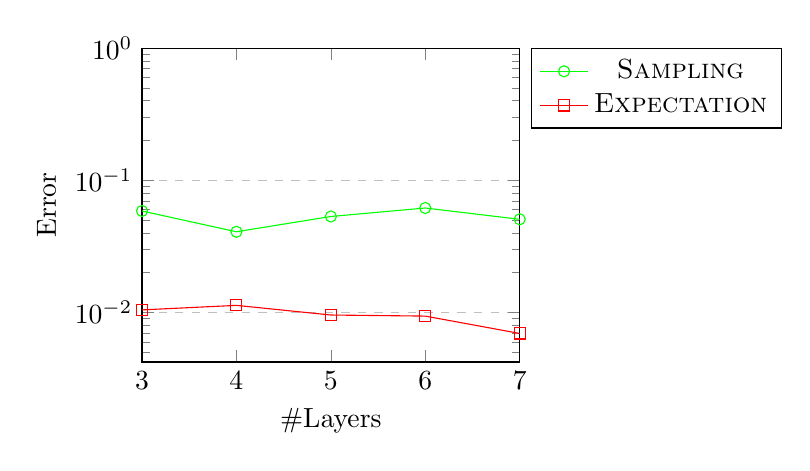
\begin{tikzpicture}
	\begin{axis}[
	scale=0.7,
	ymode = log,
	xlabel={\#Layers},
	ylabel near ticks,
	ylabel={Error},
	xmin=3, xmax=7,
	ymin=0, ymax=1,
	legend pos=outer north east,
	ymajorgrids=true,
	grid style=dashed,
	]




	\addplot[
	color=green,
	mark=o,
	]
	coordinates {
        (3,0.058648406)
        (4,0.040836635)
        (5,0.053282065)
        (6,0.061770479)
        (7,0.05073542)




	};
	\addlegendentry{\sampling}

	\addplot[
	color=red,
	mark=square,
	]
	coordinates {
        (3,0.010470007)
        (4,0.01132907)
        (5,0.009574956)
        (6,0.009398957)
        (7,0.006946578)



	};
	\addlegendentry{\expectation}

	\end{axis}
	\end{tikzpicture}
	\caption{Error comparison of all heuristic algorithms for different number of layers, deadline of $0.25\cdot maxd$ seconds and real data distribution}\label{RealDataNoesDD4Error}
\end{figure}

\begin{figure}[h!]
	\scriptsize
	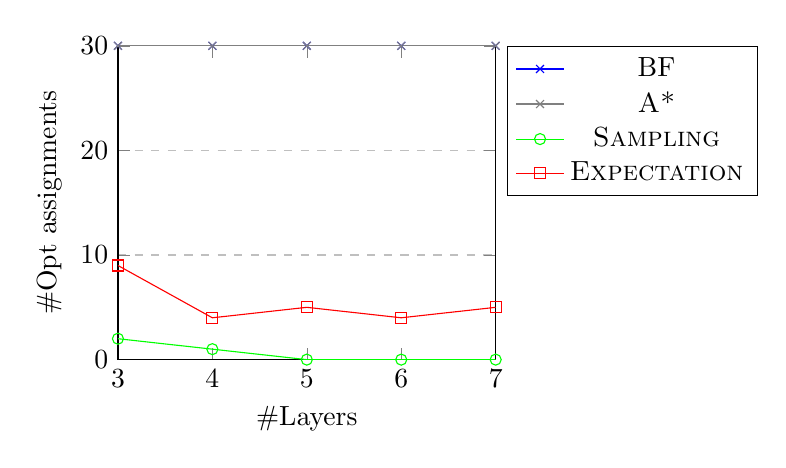
\begin{tikzpicture}
	\begin{axis}[
	scale=0.7,
	xlabel={\#Layers},
	ylabel near ticks,
	ylabel={\#Opt assignments},
	xmin=3, xmax=7,
	ymin=0, ymax=30,
	legend pos=outer north east,
	ymajorgrids=true,
	grid style=dashed,
	]

	\addplot[
	color=blue,
	mark=x,
	]
	coordinates {
		(3 , 30)
		(4 , 30)
		(5 , 30)
		(6 , 30)
		(7 , 30)

	};
	\addlegendentry{BF}

	\addplot[
	color=gray,
	mark=x,
	]
	coordinates {
		(3 , 30)
		(4 , 30)
		(5 , 30)
		(6 , 30)
		(7 , 30)

	};
	\addlegendentry{\astar}


		\addplot[
	color=green,
	mark=o,
	]
	coordinates {
		(3 , 2)
		(4 , 1)
		(5 , 0)
		(6 , 0)
		(7 , 0)

	};
	\addlegendentry{\sampling}

	\addplot[
	color=red,
	mark=square,
	]
	coordinates {
		(3 , 9)
		(4 , 4)
		(5 , 5)
		(6 , 4)
		(7 , 5)

	};
	\addlegendentry{\expectation}

	\end{axis}
	\end{tikzpicture}
	\caption{Number of optimal assignments comparison of all heuristic algorithms for different number of layers, deadline of $0.25\cdot maxd$ seconds and real data distribution}\label{RealDataNoesDD4Error}
\end{figure}

\begin{figure}[h!]
	\scriptsize
	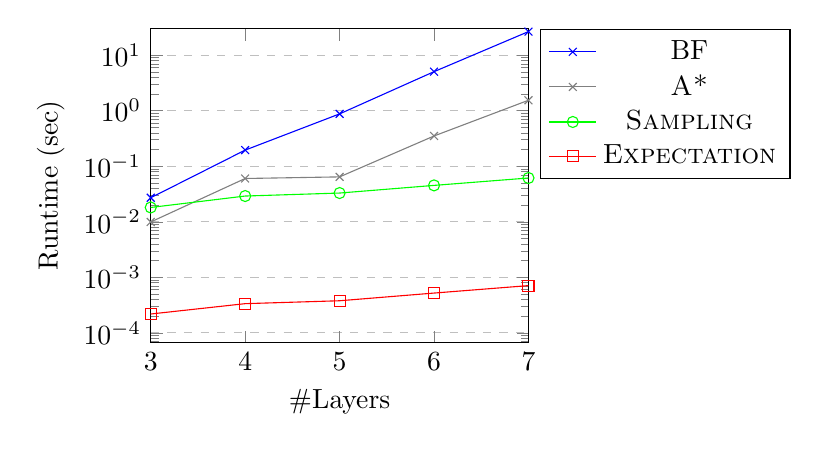
\begin{tikzpicture}
	\begin{axis}[
	scale=0.7,
	ymode = log,
	xlabel={\#Layers},
	ylabel near ticks,
	ylabel={Runtime (sec) },
	xmin=3, xmax=7,
	ymin=0, ymax=30,
	legend pos=outer north east,
	ymajorgrids=true,
	grid style=dashed,
	]

	\addplot[
	color=blue,
	mark=x,
	]
	coordinates {
        (3, 0.027072644)
        (4,0.195398919)
        (5,0.877515165)
        (6,5.055012592)
        (7,26.63227708)

	};
	\addlegendentry{BF}

	\addplot[
	color=gray,
	mark=x,
	]
	coordinates {
        (3,0.009916568)
        (4,0.060187419)
        (5,0.06435198)
        (6,0.350998553)
        (7,1.544047658)



	};
	\addlegendentry{\astar}


		\addplot[
	color=green,
	mark=o,
	]
	coordinates {
        (3,0.018108805)
        (4,0.029080073)
        (5,0.03292222)
        (6,0.045208732)
        (7,0.061459295)



	};
	\addlegendentry{\sampling}

	\addplot[
	color=red,
	mark=square,
	]
	coordinates {
        (3,0.000218225)
        (4,0.000335201)
        (5,0.0003781)
        (6,0.000520102)
        (7,0.000708803)

	};
	\addlegendentry{\expectation}

	\end{axis}
	\end{tikzpicture}
	\caption{Run time comparison of all heuristic algorithms for different number of layers, deadline of $0.25\cdot maxd$ seconds and real data distribution}\label{RealDataNoesDD4Error}
\end{figure}}










\section{Conclusion and Future Work}

We introduced the \samd problem of assigning suppliers to tasks so as to maximize the probability to meet a given project deadline. Several algorithms were proposed. Two suboptimal algorithms, \sampling and \expectation, and an optimal \astar-based algorithm. %that constitutes the highlight of our work.
Experimental evaluation on synthetic data as well as data collected from real software projects showed promising trends for our \astar-based approach that on the one hand, finds better solutions than the heuristic methods in many instances, and on the other hand, significantly outperforms the brute-force approach in terms of run-time.
We believe that the presented \samd problem is a challenging problem that can bridge the gap between the research areas of Artificial Intelligence and Project Management. In future research it will be interesting to see how \samd can be extended to allow solving projects with parallel tasks, which are common in many real-world projects.
For future work, one may consider using approximations of computations of $M(\cdot)$.
This will compromise the optimality of the algorithm, but will enable using the (now suboptimal) \astar-based approach to much larger problems.




\begin{comment}
\section{Bounded-Suboptimal Search}

Bounded-suboptimal search algorithms are search algorithm that accept a parameter $\epsilon$ and return a solution whose cost is at most $1+\epsilon$ times the cost of an optimal solution.
In the case of a maximization problem,
such algorithm return a solution whose utility is at least the utility of an optimal solution divided by $1+\epsilon$.
Weighted \astar (w\astar) is a classic example of a bounded-suboptimal search algorithm~\cite{pohl}.
w\astar is a best-first that expands in every iteration the node with the smallest $g+(1+\epsilon)\cdot h$. Explicit estimation search (EES)~\cite{thayer} and Dynamic Potential Search~\cite{gilon} are more modern examples of bounded-suboptimal search algorithms.

Some of these algorithms relay on a separation between the $g$ value and the $h$ value of a node, which is less relevant in our context.
$A^*_\epsilon$ is an algorithmic framework for bounded-suboptimal search algorithms that is particularly useful for cases where such a separation is not natural. We explain first $\astar_\epsilon$ for minimization problems, and then explain its translation to maximization problems.

Throughout its execution, $A^*_\epsilon$ maintains a lower bound on the optimal solution cost, by
keeping track of the smallest $g+h$ value in OPEN.
We denote this value by $f_{min}$. Formally,
$f_{min}=\min_{n\in OPEN} g(n)+h(n)$. If $h$ is admissible, then $f_{min}$ is a lower bound on the cost of an optimal solution. Note that $f_{min}$ may increase or decrease throughout the search, since the set of nodes in OPEN changes. Thus, to maintain the tightest lower bound we update the value of $f_{min}$ after every iteration only if it increase.
$A^*_\epsilon$ maintains a secondary data structure called FOCAL that contains all nodes in OPEN for which their $g+h$ is smaller than or equal to $(1+\epsilon)\cdot f_{min}$. Then, it chooses to expand in every iteration a single node from OPEN.
For example, $A^*_\epsilon$ may choose to expand the node in FOCAL with the smallest $h$ value, as it is estimated to be closer to a goal.


In the context of \samd, we will maintain $U_{max}$ to be the maximal $U$ value in OPEN, i.e.,
$U_{max}=\max_{n\in OPEN} U(n)$. Here, we will check $U_{max}$ after every iteration, and update it if $\max_{n\in OPEN}$ is smaller than the current $U_{max}$.
In FOCAL, we will have every node $n\in OPEN$ for which $U(n)\geq \frac{U_{max}}{(1+\epsilon)}$.
Among these nodes, we choose to expand the supplier assignment that is closest to be a full assignment.
[[here we need some kind of (not admissible) heuristic way of choosing, I propose the following simple thing]]
Note that after every expansion, the set of nodes in FOCAL may change, since new nodes are added and removed from OPEN, and $U_{max}$ may change.

\section{Complexity results}\label{sec:complexity}

We show that the SAMD problem is NP-hard,
even for a set of suppliers that have a constant duration time.
\begin{observation}
 For an instance of \samd, $M(T, \varphi, d) = Pr\left(\sum_{t\in T} X_{\varphi(t)}\leq d\right) =F_{\sum_{t\in T} X_{\varphi(t)}}(d)$
\end{observation}
For an instance of \samd $\langle T, S, X, d\rangle$,
 where $T$ is an ordered set of tasks,
 $S$ is a set of suppliers,
 $X$ is the set of random variables, one for each supplier, that represents the task completion time of this suppliers,
 and $d$ is the project deadline. We can describe \samd as a weighted directed acyclic graph (DAG) $G(T\cup g,S,X)$. The nodes in $G$ are the tasks $T$ in addition to a goal node $g$. The edges are the suppliers $S$ such that from every task $t\in T$ the outgoing edges are only the subset of suppliers that can perform task $t$ (the ongoing edges to $g$ are the outgoing edges of $t_n$). The weights are the distributions $X$ associated to each supplier. Lets look at a simplified version of \samd where $\forall X_i\in X, 0\leq i\leq |X|$ is given in the form of $Pr(X_i=x)=1$. In this simplified version, it is suffice to assume that every edge is weighted by a number.

\begin{lemma}
Given an instance of \samd $\langle T, S, X, d\rangle$ formalized as a graph $G(T,S,X)$ and $X$ is in the form of $\forall X_i\in X, Pr(X_i=x)=1$. Then, deciding whether there is a simple path $p$ between $t_1$ to $g$ where the weights on the edges sums to $d$ is NP-Hard.
\end{lemma}

\begin{proof} By reduction from \textsc{SubsetSum}~\cite[problem number SP13]{Garey:1990:CIG:574848}. Recall that
\textsc{SubsetSum} is: given a set $S=\{s_{1},\dots,s_{n}\}$ of integers, and integer target value $T$, is there a subset of $S$ whose sum is exactly $T$?
Given an instance of \textsc{SubsetSum}, create a multi-graph with $n$ nodes and $2n$ edges. From every node $n_i$ there are two outgoing edges $e_{i,1}, e_{i,2}$ weighted by $w(e_{i,1})=s_i$ and $w(e_{i,2})=0$ and $d=T$.
By construction, there exists a subset of $S$ summing to $T$ if and only if there is a simple path $p$ from $t_1$ to $g$ such that its edges are summing to $d$.
If there is a subset $S'$ of $S$ that sums to $T$ then there is a path $p$ in $G$. If $s_i\in S'$ then the edge $e_{i,1}$ is in the path, else, edge $e_{i,2}$ in the path. We got a simple path from $t_1$ to $g$ that sums to $d$. If there is simple path $p$ in $G$ then there is a subset of $S$ that sums to $T$. We start with the empty set $S'= \emptyset $. If $e_{i,1}\in p$ then $S'\cup s_i$. If $e_{i,2}\in p$ then $s_i$ is not in $S'$. The elements in $S'$ sums to $T$.
\end{proof}
\end{comment}
\bibliographystyle{aaai}
Corporis assumenda numquam vitae ipsum quis dignissimos voluptas officiis, illo quaerat neque quia inventore fugiat repudiandae?Nostrum recusandae in quas aliquid expedita reprehenderit, autem nisi velit veniam alias unde temporibus?Aut libero laboriosam exercitationem amet, repellendus impedit rerum ducimus, officia pariatur totam amet quod quia eos repellat ipsam distinctio aut, ipsa culpa unde dolore placeat exercitationem corporis accusamus praesentium est veritatis.\clearpage
\bibliography{ijcai19}

\end{document}
